\documentclass[10pt]{beamer}

% Theme and colors
\usetheme{Madrid}
\usecolortheme{beaver}

% Packages
\usepackage{graphicx}
\usepackage{booktabs}
\usepackage{amsmath}
\usepackage{natbib}
\usepackage{tikz}

% Title information
\title{Deep Learning: A Retrospective}
\subtitle{Reading LeCun, Bengio, and Hinton (Nature, 2015)}
\author{Your Name}
\institute{STAT 3494W}
\date{\today}

% Begin document
\begin{document}

% Title slide
\begin{frame}
    \titlepage
\end{frame}

% Outline slide
\begin{frame}{Outline}
    \tableofcontents
\end{frame}

% Include sections
\section{Introduction}

% Slide 2 - The Paper
\begin{frame}{The Paper}
    \begin{columns}
        \column{0.5\textwidth}
        % TODO: Add image of Nature cover or paper header
        % \includegraphics[width=\textwidth]{figures/nature_cover}
        
        \column{0.5\textwidth}
        \begin{itemize}
            \item \textbf{Published:} Nature, 2015
            \item \textbf{Authors:} LeCun, Bengio, Hinton
            \item \textbf{Citations:} 70,000+
        \end{itemize}
    \end{columns}
    
    \vspace{1em}
\end{frame}

% Slide 3 - Why Should We Trust These People?
\begin{frame}{Why Should We Trust These People?}
    \begin{itemize}
        \item \textbf{Three researchers, three legends}
        \item \textbf{Turing Award 2018} - for their work on deep learning
        \item \textbf{Nobel Prize in Physics 2024} - Hinton \& Hopfield
    \end{itemize}
    
    \vspace{1em}
\end{frame}

\section{Why Does This Paper Exist?}

% Slide 4 - The AI Hype Cycle
\begin{frame}{The AI Hype Cycle}
    % TODO: Make this better or add a real graphic. Currently missing a lot.
    \begin{itemize}
        \item \textbf{1950s--60s:} Hype cycle 1 - early AI optimism
        \item \textbf{1970s:} AI Winter 1 - symbolic AI hits limits
        \item \textbf{1980s:} Expert systems - hype cycle 2
        \item \textbf{1990s:} AI Winter 2 - expert systems fail
        \item \textbf{2000s:} ML revival - SVMs, kernel methods dominate
        \item \textbf{2012:} Something changes...
    \end{itemize}
\end{frame}

% Slide 5 - The Current landscape
\begin{frame}{The Current landscape (2015)}
    
    \vspace{1em}
    \begin{quote}
    \end{quote}
    
    \vspace{1em}
\end{frame}

% Slide 6 - What the Paper Is Actually Doing
\begin{frame}{What the Paper Is Actually Doing}
    \begin{itemize}
        \item \textbf{Not} just a technical summary
        \item A \textbf{persuasion document} written by true believers with receipts
        \item They're selling something they \textit{know} is real
    \end{itemize}
    
    \vspace{1em}
\end{frame}

% Slide 7 - Road Map
\begin{frame}{Road Map}
    \begin{enumerate}
        \item \textbf{The Basics} - Backpropagation
        \item \textbf{CNNs} - Convolutional Neural Networks
        \item \textbf{RNNs} - Recurrent Neural Networks
        \item \textbf{Predictions} - What did they predict?
        \item \textbf{Transformers} - What happened next?
    \end{enumerate}
\end{frame}

\section{The Basics: Deep Learning}

% Slide 8 - The Core Idea
\begin{frame}{The Core Idea}
    \begin{itemize}
        \item Replace \textbf{hand-engineered features} with \textbf{trainable multilayer networks}
        \item Why this matters: feature engineering was the bottleneck
    \end{itemize}
    
    \vspace{1em}
    % TODO: Add diagram: raw input → layers → output
    \begin{center}
        \texttt{Raw Input → Layer 1 → Layer 2 → ... → Output}
    \end{center}
\end{frame}

% Slide 9 - Meet Geoffrey Hinton
\begin{frame}{Meet Geoffrey Hinton}
    \begin{columns}
        \column{0.4\textwidth}
        % TODO: Add photo
        % 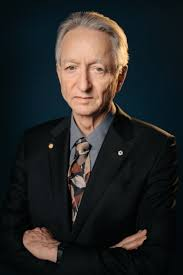
\includegraphics[width=\textwidth]{figures/hinton}
        
        \column{0.6\textwidth}
        \begin{itemize}
            \item Co-author of the \textbf{1986 backpropagation paper}
            \item Invented \textbf{Boltzmann machines} (1985)
            \item \textbf{Nobel Prize in Physics 2024}
        \end{itemize}
    \end{columns}
    
    \vspace{1em}
    \textit{``One of the authors literally helped invent what we're about to explain.''}
\end{frame}

% Slide 10 - Backpropagation
\begin{frame}{Backpropagation}
    % TODO: Add feed-forward network diagram
    
    \begin{enumerate}
        \item \textbf{Forward pass:} Input → through layers → output
        \item \textbf{Compute loss:} How wrong are we?
        \item \textbf{Backward pass:} Propagate gradients back through layers
        \item \textbf{Update weights:} Adjust in direction that reduces error
    \end{enumerate}
    
    \vspace{1em}
    \textbf{ReLU:} Fastest activation function - what the paper recommends
    
    % TODO: Add Python code example here
\end{frame}

% Slide 11 - Stochastic Gradient Descent
\begin{frame}{Stochastic Gradient Descent}
    \begin{itemize}
        \item The optimization engine
        \item Discovered by multiple groups in the 70s and 80s
        \item Including Hinton's group
    \end{itemize}
    
    \vspace{1em}
    \begin{quote}
        ``This simple procedure usually finds a good set of weights surprisingly quickly.''
    \end{quote}
\end{frame}

% Slide 12 - "But Does it Actually Work?"
\begin{frame}{``But Does it Actually Work?''}
    The saddle point rebuttal:
    
    \begin{quote}
        ``The landscape is packed with a combinatorially large number of saddle points where the gradient is zero, and the surface curves up in most dimensions and curves down in the remainder.''
    \end{quote}
    
    \vspace{1em}
    \textbf{Direct answer to the skeptics.}
    
    The authors know exactly what objection you just had.
\end{frame}

% Slide 13 - The 2006 Breakthrough
\begin{frame}{The 2006 Breakthrough}
    \begin{itemize}
        \item \textbf{CIFAR group} - first model to detect features \textit{without labeled data}
        \item Worked around limitations: small datasets, no ReLU, poor GPU support
        \item \textbf{Proved deep learning was worth pursuing}
    \end{itemize}
    
    \vspace{1em}
    \textbf{Reveal:} The authors don't even mention that \textit{they were the ones who did this.}
    
    \vspace{1em}
    Led to first commercial win: \textbf{speech recognition on Android by 2012}
\end{frame}

\section{CNNs and ImageNet}

% Slide 14 - Meet Yann LeCun
\begin{frame}{Meet Yann LeCun}
    \begin{columns}
        \column{0.4\textwidth}
        % TODO: Add photo
        % 
\includegraphics[width=\textwidth]{figures/lecun}
        
        \column{0.6\textwidth}
        \begin{itemize}
            \item \textbf{Invented CNNs} (LeNet)
            \item Bank check recognition system
            \item Reading \textbf{10\% of all US checks} by late 1990s
        \end{itemize}
    \end{columns}
    
    \vspace{1em}
    \textit{``Another author. Another invention we're about to explain.''}
\end{frame}

% Slide 15 - What is a CNN?
\begin{frame}{What is a CNN?}
    \textbf{The problem:} Standard networks ignore spatial structure
    
    \vspace{1em}
    \textbf{The solution:} Convolutional Neural Networks
    \begin{itemize}
        \item Convolution layers - detect local features
        \item Pooling layers - reduce spatial dimensions
        \item Feature maps - hierarchical representations
    \end{itemize}
    
    \vspace{1em}
    \textbf{Biologically inspired} - mirrors the visual cortex
    
    % TODO: Add CNN diagram
\end{frame}

% Slide 16 - How CNNs are Trained
\begin{frame}{How CNNs are Trained}
    % TODO: Add visualization of learned filters
    
    \begin{quote}
        ``When ConvNet models and monkeys are shown the same picture, the activations of high-level units in the ConvNet explains half of the variance of random sets of 160 neurons in the monkey's inferotemporal cortex.''
    \end{quote}
    
    \vspace{1em}
    \textbf{They're not just saying it works - they're saying it works like a brain.}
\end{frame}

% Slide 17 - Early CNN Deployments
\begin{frame}{Early CNN Deployments}
    \begin{itemize}
        \item Speech recognition, OCR, handwriting recognition
        \item Microsoft deployments
        \item Face and hand detection in the early 90s
    \end{itemize}
    
    \vspace{1em}
    \textbf{``This was working for 20 years and the mainstream ignored it.''}
\end{frame}

% Slide 18 - ImageNet 2012
\begin{frame}{ImageNet 2012}
    \textbf{AlexNet enters the competition}
    
    \vspace{1em}
    \begin{itemize}
        \item \textbf{Almost halving} error rates of the best competing approach
        \item Key ingredients:
        \begin{itemize}
            \item GPUs
            \item ReLU activation
            \item Dropout regularization
            \item Data augmentation
        \end{itemize}
    \end{itemize}
    
    \vspace{1em}
    \textbf{This is the moment the mainstream could no longer ignore it.}
\end{frame}

% Slide 19 - The World Notices
\begin{frame}{The World Notices}
    \begin{quote}
        ``Companies such as Mobileye and NVIDIA are using such ConvNet-based methods in their upcoming vision systems for cars.''
    \end{quote}
    
    \vspace{1em}
    \begin{itemize}
        \item NVIDIA investing in deep learning chips
        \item Tesla self-driving cars
        \item \textit{If you read this paper in 2015 and bought NVIDIA stock...}
    \end{itemize}
    
    \vspace{1em}
    \textbf{The hype is warranted - they know it's going to work.}
\end{frame}

% Slide 20 - Why Was it Ignored for So Long?
\begin{frame}{Why Was it Ignored for So Long?}
    \begin{itemize}
        \item CNNs were largely forsaken until 2012
        \item \textbf{Despite working since the early 90s}
        \item The AI winters left scars
    \end{itemize}
    
    \vspace{1em}
    \textit{``If it works for images, what about language?''}
\end{frame}

\section{RNNs and Language}

% Slide 21 - Meet Yoshua Bengio
\begin{frame}{Meet Yoshua Bengio}
    \begin{columns}
        \column{0.4\textwidth}
        % TODO: Add photo
        % 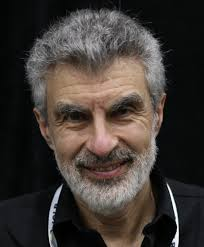
\includegraphics[width=\textwidth]{figures/bengio}
        
        \column{0.6\textwidth}
        \begin{itemize}
            \item \textbf{Most cited computer scientist globally}
            \item Most cited living scientist across all fields
            \item Neural probabilistic language model - \textbf{word embeddings}
        \end{itemize}
    \end{columns}
    
    \vspace{1em}
    \textit{``Third author. You know what's coming.''}
\end{frame}

% Slide 22 - The Language Problem
\begin{frame}{The Language Problem}
    \textbf{Old approach:} N-grams - counting symbol frequencies
    
    \vspace{1em}
    Number of possible N-grams: $V^N$ where $V$ = vocabulary size
    
    \vspace{1em}
    \begin{itemize}
        \item Brittle
        \item Slow
        \item No understanding of meaning
    \end{itemize}
\end{frame}

% Slide 23 - The Exponential Advantages
\begin{frame}{The Exponential Advantages of Deep Networks}
    Two reasons deep networks are powerful for language:
    
    \vspace{1em}
    \begin{enumerate}
        \item $n$ binary features $\rightarrow$ $2^n$ possible combinations
        
        \textit{``30 neurons can represent over a billion concepts''}
        
        \item Each layer \textbf{multiplies} expressive power exponentially
    \end{enumerate}
\end{frame}

% Slide 24 - Word Embeddings
\begin{frame}{Word Embeddings}
    \begin{itemize}
        \item \textbf{One-hot encoding:} one component = 1, rest = 0
        \item First layer creates activation patterns per word
        \item Foreshadows Word2Vec and modern embeddings
    \end{itemize}
    
    \vspace{1em}
    \textbf{Example:}
    \begin{itemize}
        \item Tuesday and Wednesday $\rightarrow$ similar vectors
        \item Sweden and Norway $\rightarrow$ similar vectors
    \end{itemize}
    
    \vspace{1em}
    \textit{``They didn't program it to learn this. It just did.''}
\end{frame}

% Slide 25 - Simple Feed Forward Language Model
\begin{frame}{Simple Feed Forward Language Model}
    \begin{itemize}
        \item Given 5 words, predict the next
        \item Works surprisingly well on:
        \begin{itemize}
            \item Small, clean datasets
            \item Large, messy real-world corpora
        \end{itemize}
    \end{itemize}
    
    \vspace{1em}
    \textbf{This was contrary to what people expected.}
\end{frame}

% Slide 26 - RNNs
\begin{frame}{Recurrent Neural Networks (RNNs)}
    \textbf{The problem:} Feed-forward networks can't handle sequences
    
    \vspace{1em}
    % TODO: Add RNN diagram (unrolled)
    
    \begin{itemize}
        \item Can translate English to French
        \item Learns semantic rules of both languages
        \item \textbf{Problem:} Vanishing gradient
    \end{itemize}
\end{frame}

% Slide 27 - LSTMs
\begin{frame}{Long Short-Term Memory (LSTM)}
    \textbf{Invented 1997}
    
    \vspace{1em}
    % TODO: Add LSTM cell diagram
    
    \begin{itemize}
        \item Cell state - long-term memory
        \item Gates - control information flow
        \item \textbf{Intuition:} Memory with a forget switch
    \end{itemize}
    
    \vspace{1em}
    The authors are bullish - and they're right.
\end{frame}

% Slide 28 - The Memory Bottleneck
\begin{frame}{The Memory Bottleneck}
    The biggest remaining problem:
    
    \vspace{1em}
    \begin{itemize}
        \item Neural networks are \textbf{stateless}
        \item Memory is inherently \textbf{stateful}
    \end{itemize}
    
    \vspace{1em}
    \textbf{Neural Turing Machines} (DeepMind, 2014)
    \begin{itemize}
        \item Differentiable Turing machine
        \item Attention-based read/write to memory
    \end{itemize}
    
    \vspace{1em}
    \textit{``They've identified the exact problem. The solution is two years away.''}
\end{frame}

\section{What They Predicted}

% Slide 29 - The Paper's Bets
\begin{frame}{The Paper's Bets}
    \textbf{2015. Let's grade their predictions.}
    
    \vspace{1em}
    \begin{enumerate}
        \item Unsupervised learning
        \item Attention mechanisms
        \item Reinforcement learning for vision
        \item Natural language understanding
    \end{enumerate}
\end{frame}

% Slide 30 - Unsupervised Learning
\begin{frame}{Prediction: Unsupervised Learning}
    \textbf{They said:} Training largely unsupervised is the path forward.
    
    \vspace{1em}
    \textbf{What happened:}
    \begin{itemize}
        \item GPT - unsupervised pretraining
        \item BERT - self-supervised learning
        \item Modern LLMs
    \end{itemize}
    
    \vspace{1em}
    \textbf{Grade: \checkmark}
\end{frame}

% Slide 31 - Attention as the Missing Piece
\begin{frame}{Prediction: Attention}
    \begin{quote}
        ``Systems that use RNNs... will become much better when they learn strategies for selectively attending to one part at a time.''
    \end{quote}
    
    \vspace{1em}
    \textbf{What happened:}
    \begin{itemize}
        \item ``Attention is All You Need'' - 2017
        \item Transformers
    \end{itemize}
    
    \vspace{1em}
    \textbf{Grade: \checkmark\checkmark}
\end{frame}

% Slide 32 - Reinforcement Learning for Vision
\begin{frame}{Prediction: Reinforcement Learning for Vision}
    \begin{quote}
        ``Human vision is an active process that sequentially samples the optic array in an intelligent, task-specific way.''
    \end{quote}
    
    \vspace{1em}
    \textbf{What happened:}
    \begin{itemize}
        \item CNN + RNN + RL
        \item DeepMind's game-playing agents
    \end{itemize}
    
    \vspace{1em}
    \textbf{Grade: \checkmark}
\end{frame}

% Slide 33 - Natural Language Understanding
\begin{frame}{Prediction: Natural Language Understanding}
    \begin{quote}
        ``Major progress will come through systems that combine representation learning with complex reasoning.''
    \end{quote}
    
    \vspace{1em}
    \textbf{What happened:}
    \begin{itemize}
        \item LLMs are impressive
        \item But still brittle on reasoning
    \end{itemize}
    
    \vspace{1em}
    \textbf{Grade: Partial \checkmark - making progress, not solved}
\end{frame}

\section{Then Transformers Happened}

% Slide 34 - 2017: A New Architecture
\begin{frame}{2017: A New Architecture}
    \textbf{Transformers}
    
    \vspace{1em}
    \begin{itemize}
        \item You've seen this before in class
        \item ``Attention is All You Need'' discards recurrence entirely
    \end{itemize}
    
    \vspace{1em}
    \textit{``Now you know what problem it was solving.''}
\end{frame}

% Slide 35 - What Transformers Got Right
\begin{frame}{What Transformers Got Right That the Paper Missed}
    \begin{itemize}
        \item The paper assumed RNNs were the right backbone for sequences
        \item Transformers showed: \textbf{you don't need recurrence at all}
        \item If attention is powerful enough
    \end{itemize}
    
    \vspace{1em}
    The memory bottleneck they identified was real - but the solution wasn't Neural Turing Machines, it was \textbf{self-attention}.
\end{frame}

% Slide 36 - What the Paper Got Right
\begin{frame}{What the Paper Got Right About Transformers}
    (Without knowing it)
    
    \vspace{1em}
    \begin{itemize}
        \item \textbf{Unsupervised pretraining:} GPT is exactly this
        \item \textbf{Attention as key mechanism:} they named it
        \item \textbf{Scale matters:} they said it, transformers proved it
    \end{itemize}
    
    \vspace{1em}
    \textit{``They predicted the destination without predicting the vehicle.''}
\end{frame}

% Slide 37 - Conclusions That Still Hold
\begin{frame}{Conclusions That Still Hold}
    \begin{itemize}
        \item Deep learning over hand-engineered features: \textbf{obviously true}
        \item Scale + data + compute: \textbf{validated completely}
        \item Representation learning as foundation: \textbf{yes}
    \end{itemize}
    
    \vspace{1em}
    \textbf{Still open:} Reasoning, grounding, true language understanding
\end{frame}

% Slide 38 - Where Are We Now
\begin{frame}{Where Are We Now}
    \begin{itemize}
        \item LLMs are extraordinary - but not AGI
        \item The paper's philosophical question still stands:
    \end{itemize}
    
    \vspace{1em}
    \begin{quote}
        ``New paradigms are needed to replace rule-based manipulation of symbolic expressions.''
    \end{quote}
    
    \vspace{1em}
    We have better tools. The question isn't answered.
\end{frame}

\section{Conclusion}

% Slide 39 - What Made This Paper Special
\begin{frame}{What Made This Paper Special}
    \begin{itemize}
        \item Not just a summary - a \textbf{persuasion document}
        \item Written by the people who \textbf{built the field}
        \item Every claim backed by work they personally did
        \item They were selling something they knew was real
    \end{itemize}
\end{frame}

% Slide 40 - The Scorecard
\begin{frame}{The Scorecard}
    \begin{table}
        \centering
        \begin{tabular}{@{}lc@{}}
            \toprule
            \textbf{Prediction} & \textbf{Outcome} \\ \midrule
            Unsupervised learning & \checkmark \\
            Attention mechanisms & \checkmark\checkmark \\
            RL for vision & \checkmark \\
            Language understanding & Partial \checkmark \\
            RNNs as backbone & $\times$ (Transformers won) \\ \bottomrule
        \end{tabular}
    \end{table}
\end{frame}

% Slide 41 - Thank You
\begin{frame}{Thank You / Questions}
    \vspace{2em}
    \begin{center}
        \Large
        \textit{``They predicted the future pretty well.}
        
        \textit{The parts they got wrong are the parts we're still working on.''}
    \end{center}
\end{frame}

% References
\section{References}

\begin{frame}{References}
    \bibliographystyle{jasa}
    \bibliography{references}{}
\end{frame}


\end{document}

%%% Local Variables:
%%% mode: latex
%%% TeX-master: t
%%% End:
